\chapter{HASIL DAN PEMBAHASAN}
\label{chap:hasil dan pembahasan}

% Ubah bagian-bagian berikut dengan isi dari pengujian dan analisis

Pada penelitian ini dilakukan 3 aspek pengerjaan dalam menjawab tujuannya, diantaranya adalah data eksperimen yang telah didapatkan dari PTDI. Kemudian validasi matematis menggunakan landasan teori yang telah disesuaikan dengan kondisi pengerjaan penelitian ini, yaitu \textit{ground resonance} helikopter. Kemudian yang terakhir adalah simulasi untuk mendukung hasil data pengukuran dan perhitungan. 

\section{Hasil Data Pengukuran dan Perhitungan}
\label{sec:hasilpengukuran}

\subsection{Hasil pengukuran getaran pada FTIS}

Hasil pengukuran data \textit{ground test} dibagi menjadi 2 bagian, seperti yang telah dijelaskan pada bagian metodologi penelitian, bahwa data yang didapatkan merupakan data pengukuran getaran pada FTIS untuk mencari \textit{damping ratio} dan pengukuran data getaran pada akseleromter untuk mendapatkan respon frekuensi dominan oleh helikopter akibat \textit{input} yang diberikan. Berikut ini merupakan grafik yang didapatkan dari masing-masing kondisi yang mengacu pada tabel \ref{tb:variasilanding}.

\begin{figure}[H]
	\centering
	\includegraphics[width=0.7\linewidth]{gambar/Condition_1.jpg}
	\caption{Grafik data hasil pengukuran kondisi 1.}
	\label{fig:condition_1}
\end{figure}

Selanjutnya merupakan grafik dengan keterangan serupa, dimana pada grafik tersebut memiliki keterangan sebagaimana pada tabel berikut:

\begin{table}[]
	\caption{Keterangan pengukuran pada grafik}
	\begin{tabular}{|c|c|c|}
		\hline
		\textit{Lateral cyclic displacement (\%)} & \textit{Longitudinal cyclic displacement} & Pedal displacement (\%)           \\ \hline
		\textit{Roll (deg)}                       & \textit{Pitch (deg)}                      & \textit{Heading (deg)}            \\ \hline
		\textit{Rate of roll (deg/s)}             & \textit{Rate of Pitch (deg/s)}            & \textit{Rate of Yaw (deg/s)}      \\ \hline
		\textit{Acceleration-x ($m/s^2$)}         & \textit{Acceleration-y ($m/s^2$)}         & \textit{Acceleration-z ($m/s^2$)} \\ \hline
	\end{tabular}
\end{table}

Posisi dari masing-masing keterangan berkorelasi dengan posisi pada grafik yang diberikan, contoh: pada bagian awal, dari arah kiri terdapat keterangan "\textbf{\textit{Lateral Cyclic Displacement (\%)}}" maka grafik pada posisi tersebut merepresentasikan "\textbf{\textit{Lateral Cyclic Displacement (\%)}}", begitu seterusnya.

\begin{figure}[H]
	\begin{subfigure}{0.49\textwidth}
		\centering
		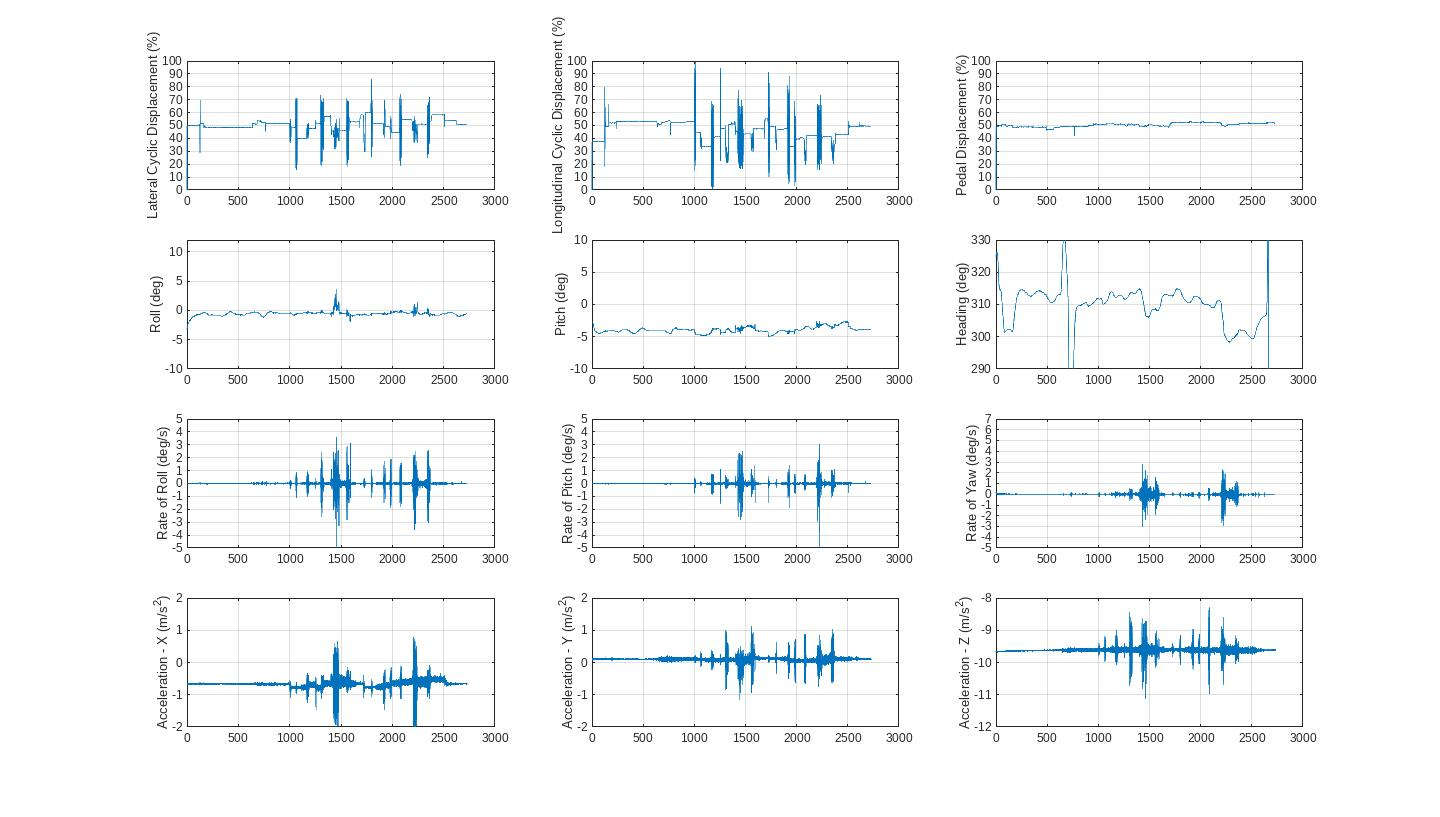
\includegraphics[width=\linewidth]{gambar/Condition_2.jpg}
		\caption{}
		\label{fig:condition_2}
	\end{subfigure}
	\centering
	\begin{subfigure}{0.51\textwidth}
		\centering
		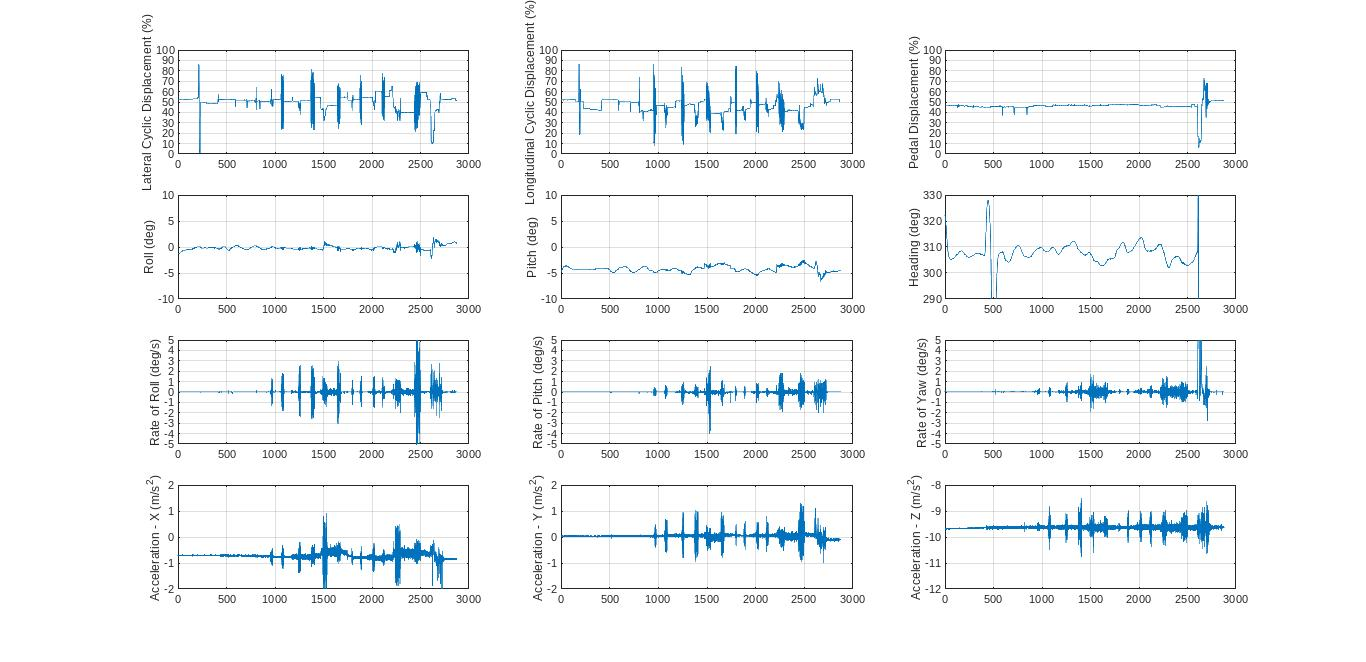
\includegraphics[width=\linewidth]{gambar/Condition_3.jpg}
		\caption{}
		\label{fig:condition_3}
	\end{subfigure}
	\caption{(a) Grafik data pengukuran pada kondisi-2 (b) Grafik data pengukuran pada kondisi-3.}
\end{figure}

\begin{figure}[H]
	\begin{subfigure}{0.49\textwidth}
		\centering
		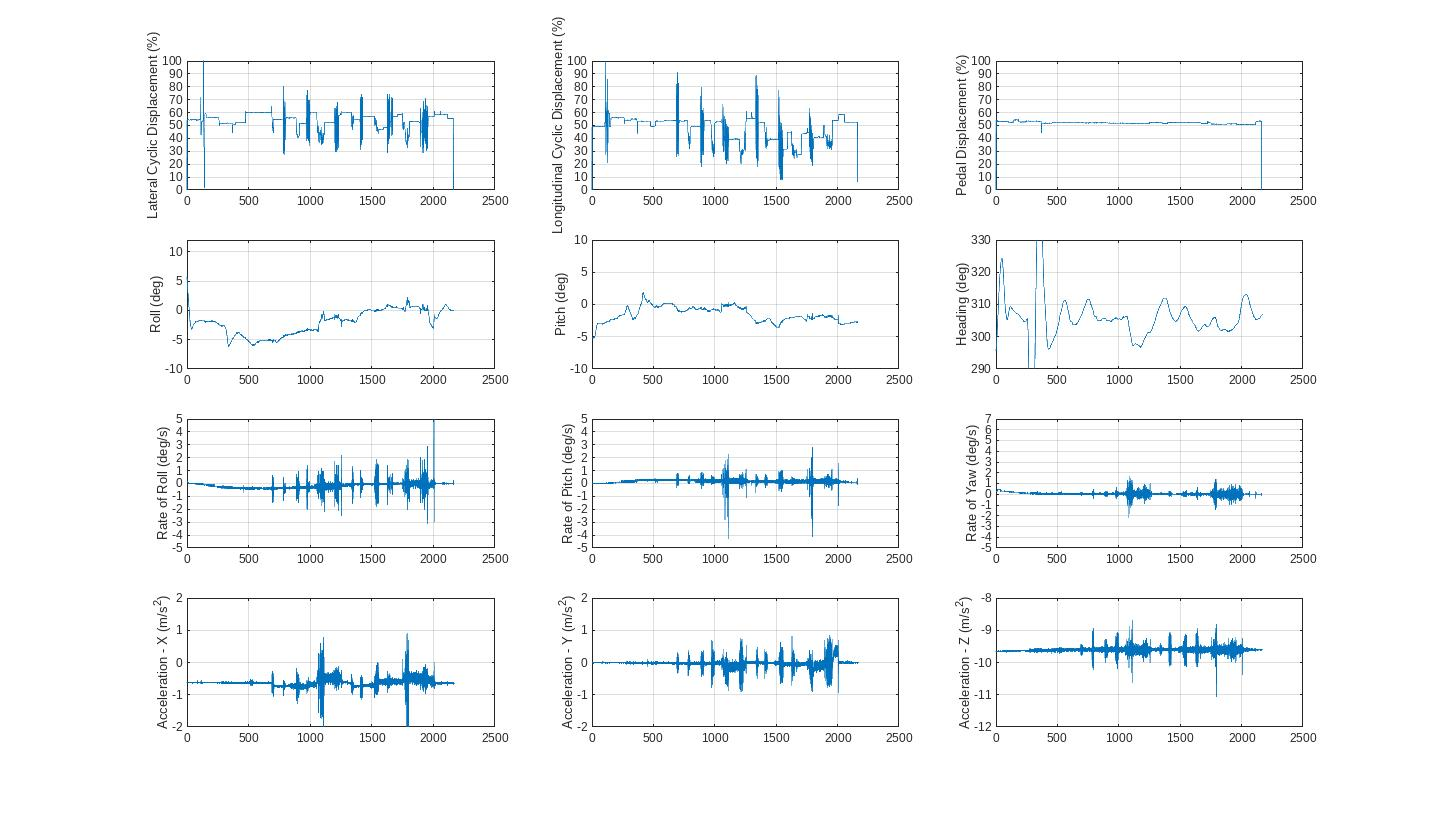
\includegraphics[width=\linewidth]{gambar/Condition_4.jpg}
		\caption{}
		\label{fig:condition_4}
	\end{subfigure}
	\centering
	\begin{subfigure}{0.49\textwidth}
		\centering
		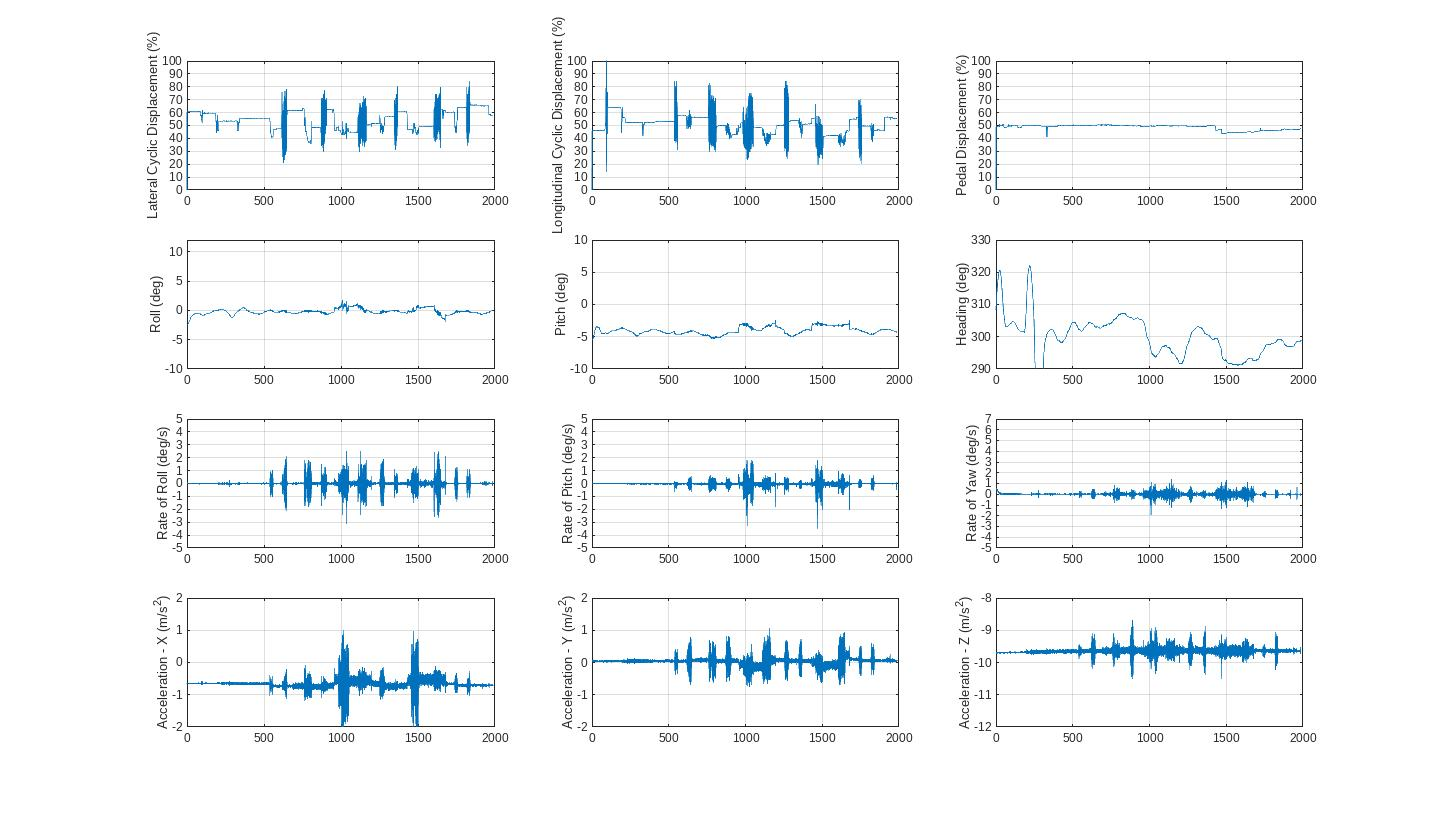
\includegraphics[width=\linewidth]{gambar/Condition_5.jpg}
		\caption{}
		\label{fig:condition_5}
	\end{subfigure}
	\caption{(a) Grafik data pengukuran pada kondisi-4 (b) Grafik data pengukuran pada kondisi-5.}
\end{figure}

\begin{figure}[H]
	\begin{subfigure}{0.5\textwidth}
		\centering
		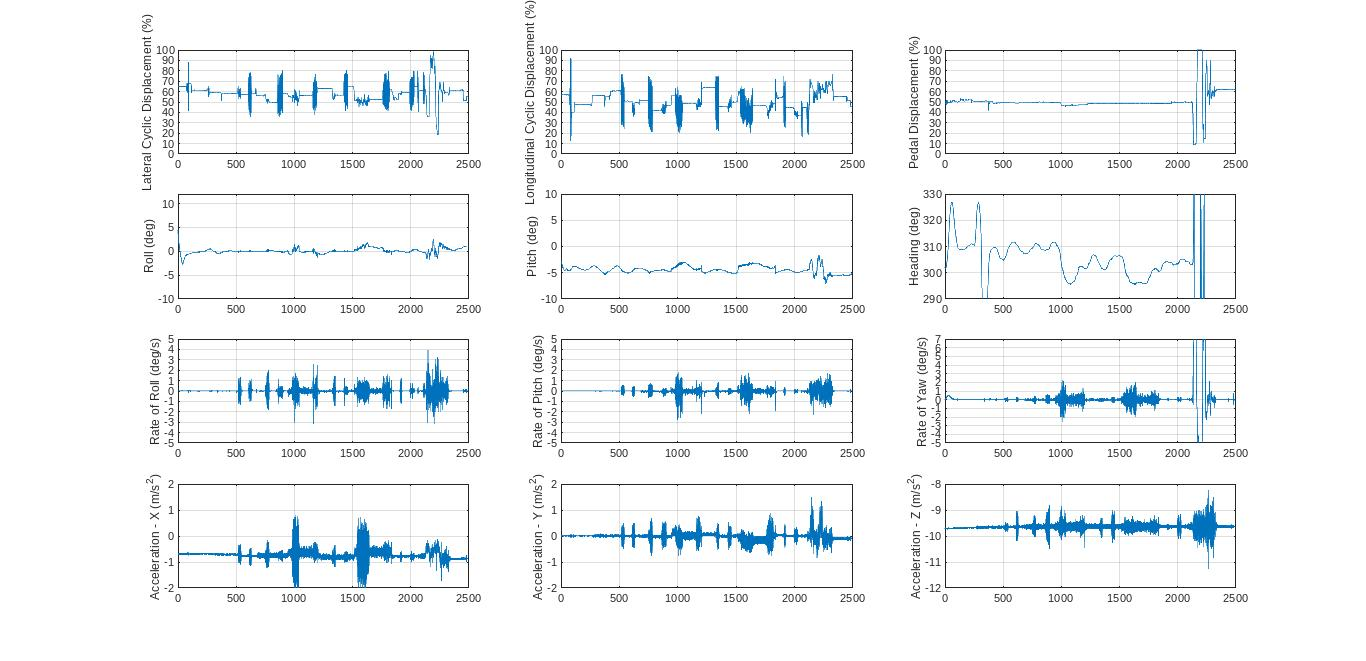
\includegraphics[width=\linewidth]{gambar/Condition_6.jpg}
		\caption{}
		\label{fig:condition_6}
	\end{subfigure}
	\centering
	\begin{subfigure}{0.49\textwidth}
		\centering
		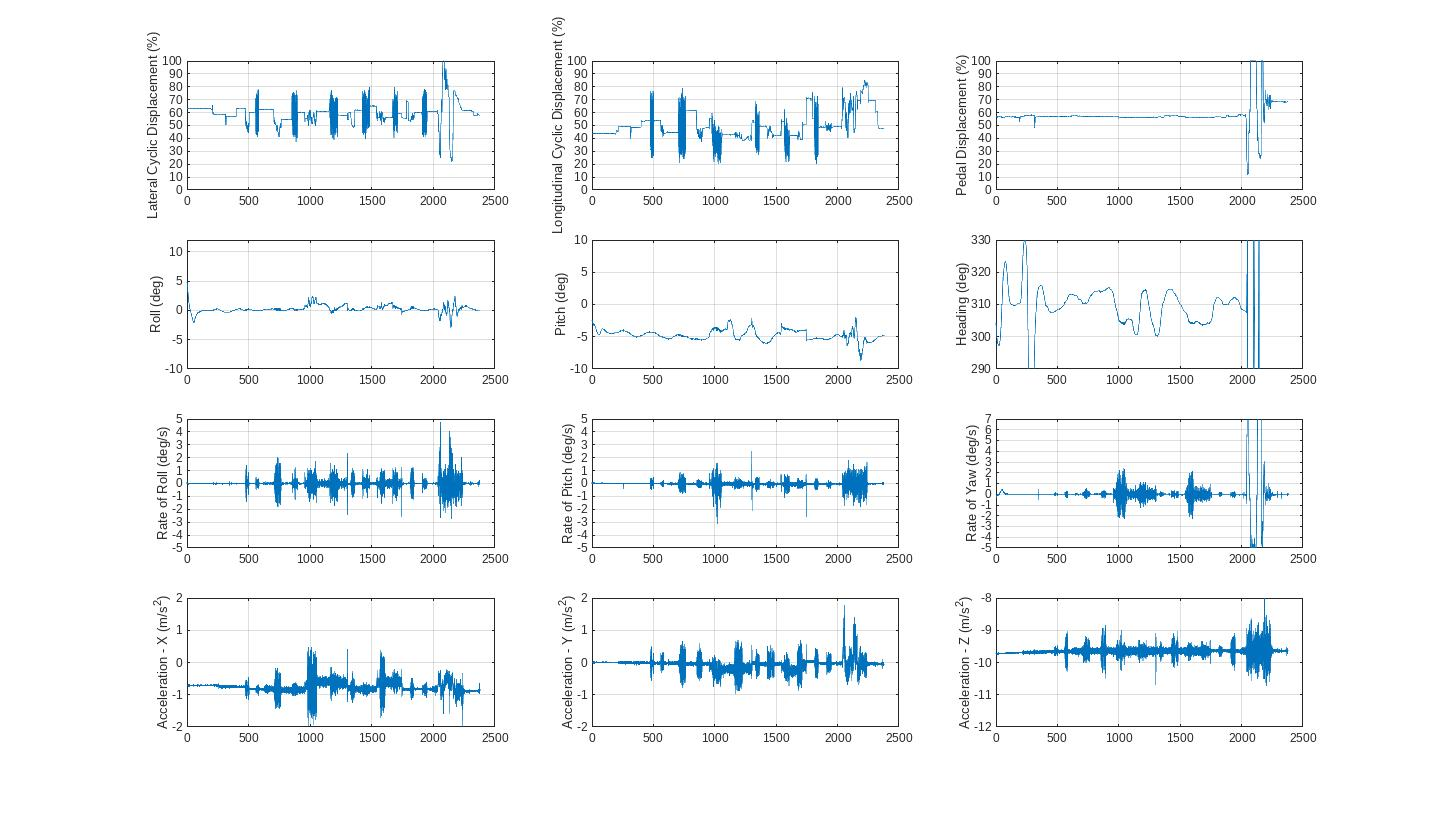
\includegraphics[width=\linewidth]{gambar/Condition_7.jpg}
		\caption{}
		\label{fig:condition_7}
	\end{subfigure}
	\caption{(a) Grafik data pengukuran pada kondisi-6 (b) Grafik data pengukuran pada kondisi-7.}
\end{figure}

\begin{figure}[H]
	\begin{subfigure}{0.49\textwidth}
		\centering
		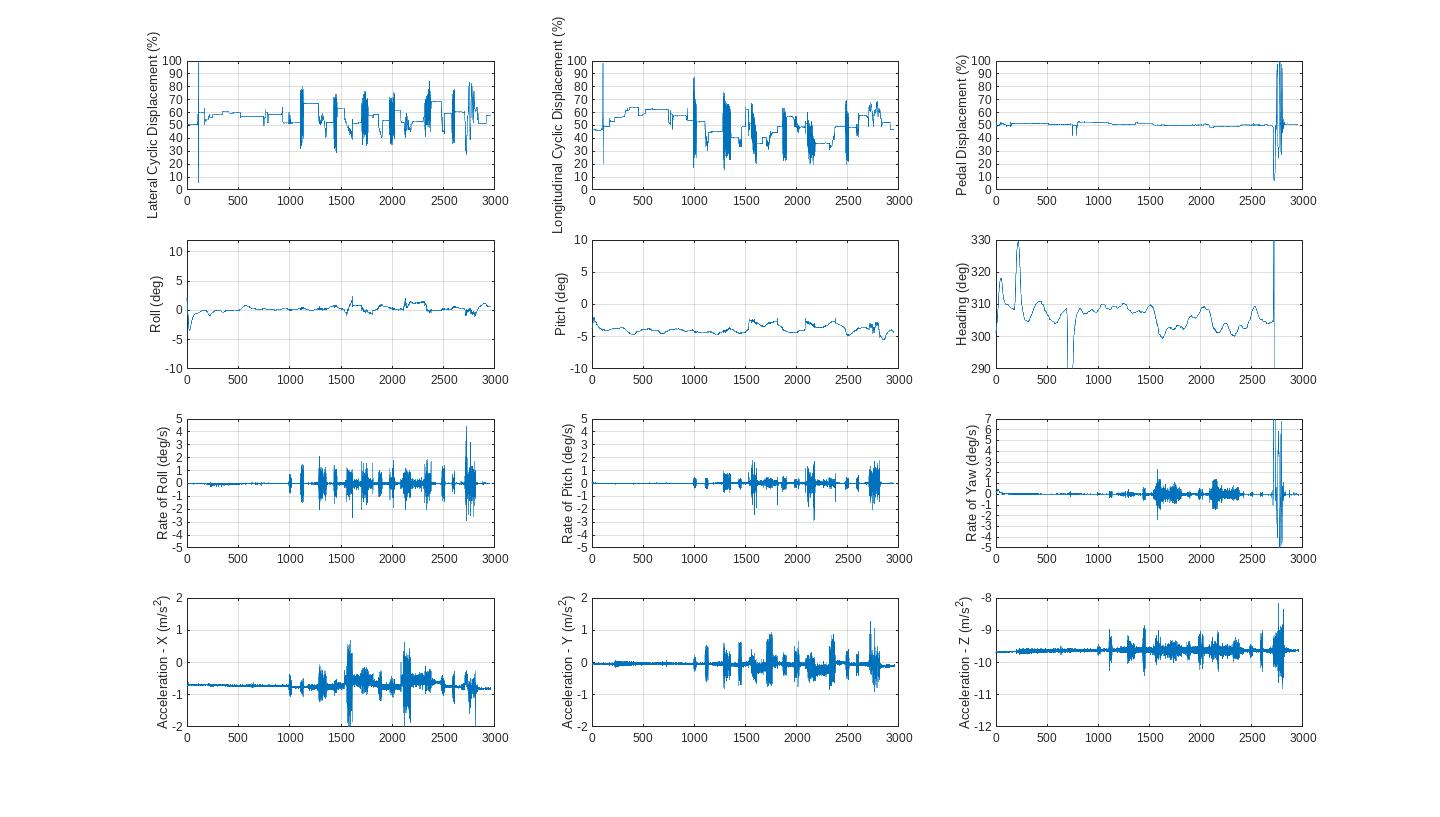
\includegraphics[width=\linewidth]{gambar/Condition_8.jpg}
		\caption{}
		\label{fig:condition_8}
	\end{subfigure}
	\centering
	\begin{subfigure}{0.49\textwidth}
		\centering
		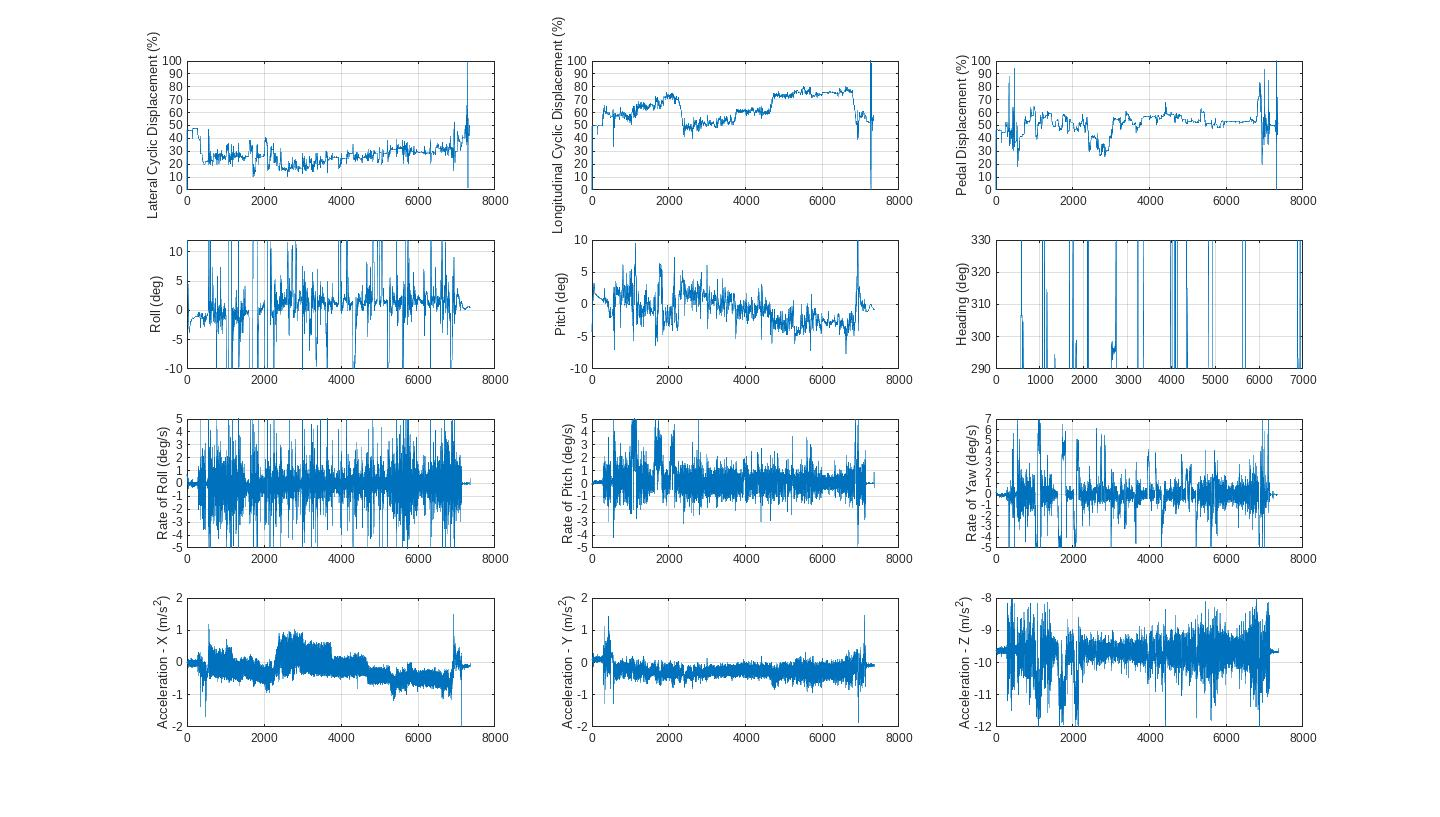
\includegraphics[width=\linewidth]{gambar/Condition_9.jpg}
		\caption{}
		\label{fig:condition_9}
	\end{subfigure}
	\caption{(a) Grafik data pengukuran pada kondisi-8 (b) Grafik data pengukuran pada kondisi-9.}
\end{figure}

\begin{figure}[H]
	\begin{subfigure}{0.49\textwidth}
		\centering
		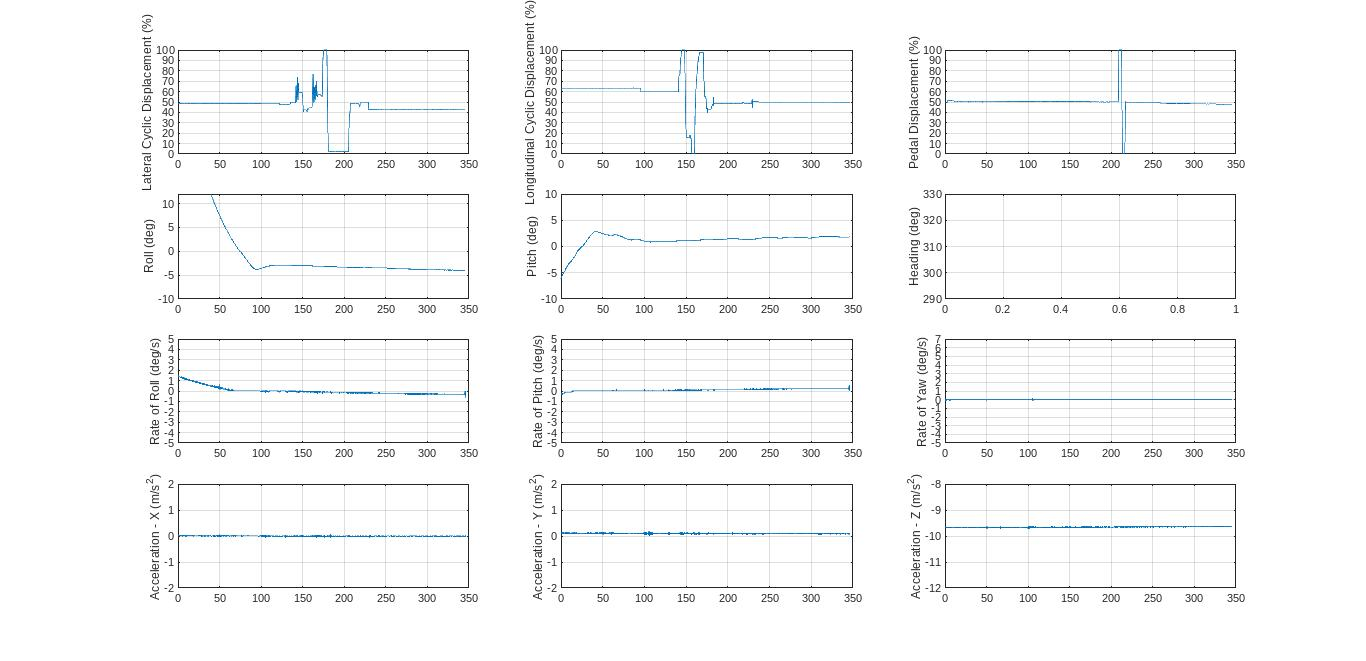
\includegraphics[width=\linewidth]{gambar/Condition_10.jpg}
		\caption{}
		\label{fig:condition_10}
	\end{subfigure}
	\centering
	\begin{subfigure}{0.49\textwidth}
		\centering
		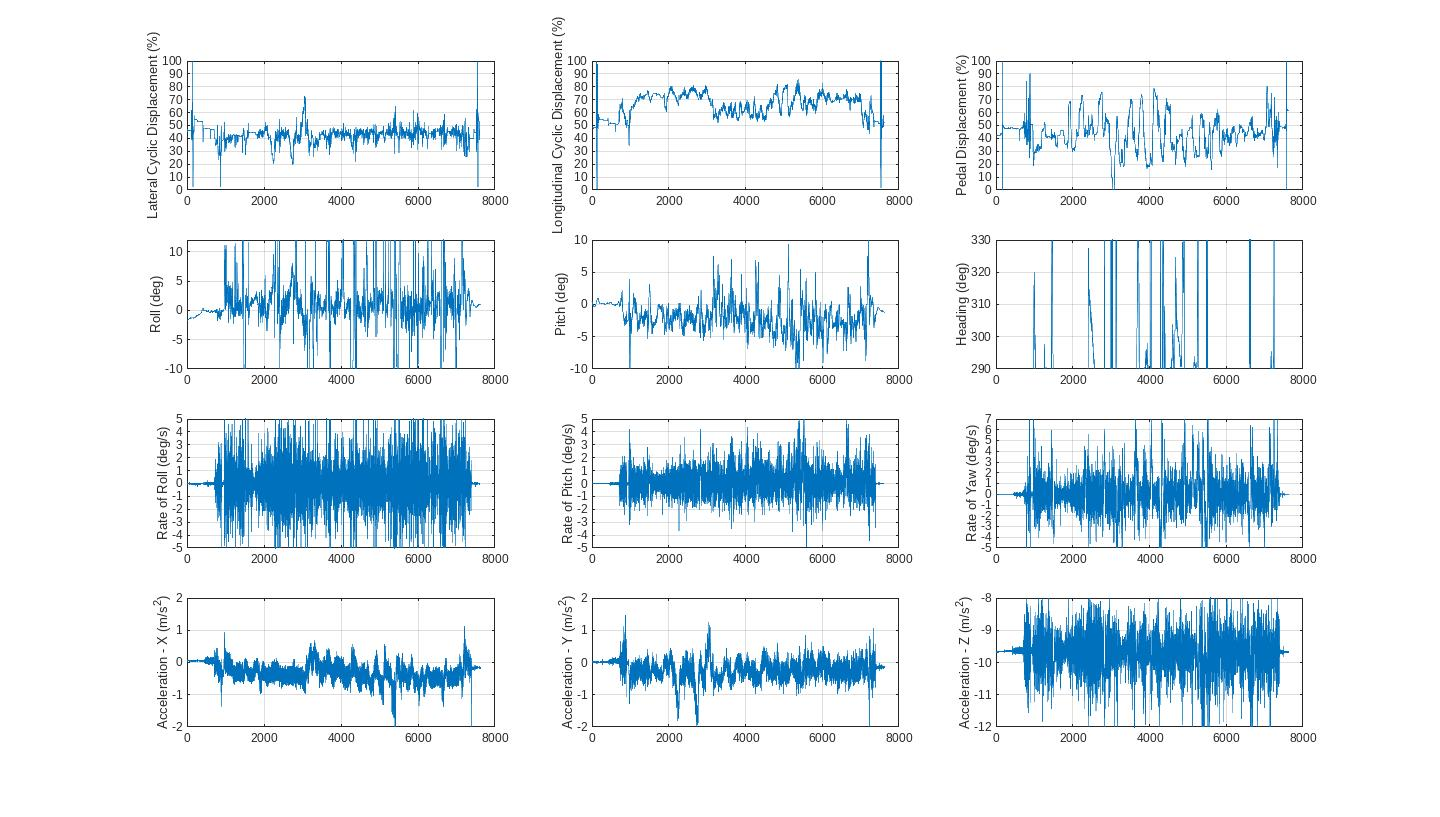
\includegraphics[width=\linewidth]{gambar/Condition_11.jpg}
		\caption{}
		\label{fig:condition_11}
	\end{subfigure}
	\caption{(a) Grafik data pengukuran pada kondisi-10 (b) Grafik data pengukuran pada kondisi-11.}
\end{figure}

Dari grafik diatas selanjutnya akan dibagi menjadi beberapa segmen yang sesuai dengan variasi input yang telah diberikan pada tabel \ref{tb:variasi_input}. Untuk menghitung besarnya \textit{damping ratio}, digunakan rumus (akan dilengkapi nanti di BAB 2). Dari formulasi tersebut didapatkan nilai kuantifikasi terhadap \textit{damping ratio} helikopter. Akan tetapi sebelumnya diperlukan sebuah pengamatan untuk melihat apakah helikopter masih memberikan respon meskipun \textit{input} yang diberikan telah berhenti. Maka dari tabel berikut ini menjelaskan pada kondisi serta variasi apa saja yang masih memberikan respon meskipun \textit{input} yang diberikan telah berhenti.

Pada bagian tabel \ref{tb:waktupeluruhan} informasi ( - ), menandakan bahwa helikopter tidak memberikan respon terhadap \textit{input} yang diberikan. Sedangkan informasi yang berisi ( TC : Teredam Cepat) menandakan bahwa respon yang diberikan helikopter langsung kembali ke posisi setimbang dengan cepat. Sehingga didapatkan informasi berupa nilai maksimum dan minimum serta nilai-nilai lain dari waktu peluruhan untuk masing-masing kondisi. 

\begin{table}[]
	\caption{Waktu peluruhan untuk setiap kondisi}
	\label{tb:waktupeluruhan}
	\begin{tabular}{|c|ccccccccccc|}
		\hline
		& \multicolumn{11}{c|}{Waktu peluruhan amplitudo (s)} \\ \cline{2-12} 
		\multirow{-2}{*}{Variasi \textit{input}} & \multicolumn{1}{c|}{1} & \multicolumn{1}{c|}{2} & \multicolumn{1}{c|}{3} & \multicolumn{1}{c|}{4} & \multicolumn{1}{c|}{5} & \multicolumn{1}{c|}{6} & \multicolumn{1}{c|}{7} & \multicolumn{1}{c|}{8} & \multicolumn{1}{c|}{9} & \multicolumn{1}{c|}{10} & 11 \\ \hline
		FILO & \multicolumn{1}{c|}{\cellcolor[HTML]{FFCCC9}-} & \multicolumn{1}{c|}{17.22} & \multicolumn{1}{c|}{10.97} & \multicolumn{1}{c|}{\cellcolor[HTML]{FFFFC7}TC} & \multicolumn{1}{c|}{\cellcolor[HTML]{FFFFC7}TC} & \multicolumn{1}{c|}{\cellcolor[HTML]{FFCCC9}-} & \multicolumn{1}{c|}{10.97} & \multicolumn{1}{c|}{\cellcolor[HTML]{FFFFC7}TC} & \multicolumn{1}{c|}{\cellcolor[HTML]{FFFFC7}TC} & \multicolumn{1}{c|}{8.51} & \cellcolor[HTML]{FFFFC7}TC \\ \hline
		FILA & \multicolumn{1}{c|}{\cellcolor[HTML]{FFCCC9}-} & \multicolumn{1}{c|}{9.92} & \multicolumn{1}{c|}{5.51} & \multicolumn{1}{c|}{5.35} & \multicolumn{1}{c|}{\cellcolor[HTML]{FFFFC7}TC} & \multicolumn{1}{c|}{\cellcolor[HTML]{FFFFC7}TC} & \multicolumn{1}{c|}{6.37} & \multicolumn{1}{c|}{6.39} & \multicolumn{1}{c|}{7.33} & \multicolumn{1}{c|}{6.98} & \cellcolor[HTML]{FFCCC9}- \\ \hline
		FFLO & \multicolumn{1}{c|}{5.51} & \multicolumn{1}{c|}{17.22} & \multicolumn{1}{c|}{10.28} & \multicolumn{1}{c|}{\cellcolor[HTML]{FFFFC7}TC} & \multicolumn{1}{c|}{\cellcolor[HTML]{FFFFC7}TC} & \multicolumn{1}{c|}{\cellcolor[HTML]{FFFFC7}TC} & \multicolumn{1}{c|}{6.98} & \multicolumn{1}{c|}{\cellcolor[HTML]{FFFFC7}TC} & \multicolumn{1}{c|}{\cellcolor[HTML]{FFFFC7}TC} & \multicolumn{1}{c|}{8.25} & 7.95 \\ \hline
		FFLA & \multicolumn{1}{c|}{7.27} & \multicolumn{1}{c|}{10.97} & \multicolumn{1}{c|}{6.65} & \multicolumn{1}{c|}{\cellcolor[HTML]{FFFFC7}TC} & \multicolumn{1}{c|}{\cellcolor[HTML]{FFFFC7}Tc} & \multicolumn{1}{c|}{\cellcolor[HTML]{FFFFC7}TC} & \multicolumn{1}{c|}{\cellcolor[HTML]{FFFFC7}TC} & \multicolumn{1}{c|}{5.69} & \multicolumn{1}{c|}{9.69} & \multicolumn{1}{c|}{7.33} & 8.51 \\ \hline
		FLLO & \multicolumn{1}{c|}{\cellcolor[HTML]{FFCCC9}-} & \multicolumn{1}{c|}{4.02} & \multicolumn{1}{c|}{11.43} & \multicolumn{1}{c|}{8.92} & \multicolumn{1}{c|}{8.17} & \multicolumn{1}{c|}{\cellcolor[HTML]{FFFFC7}TC} & \multicolumn{1}{c|}{\cellcolor[HTML]{FFFFC7}TC} & \multicolumn{1}{c|}{6.63} & \multicolumn{1}{c|}{\cellcolor[HTML]{FFFFC7}TC} & \multicolumn{1}{c|}{8.48} & 6.73 \\ \hline
		FLLA & \multicolumn{1}{c|}{\cellcolor[HTML]{FFCCC9}-} & \multicolumn{1}{c|}{9.88} & \multicolumn{1}{c|}{24.07} & \multicolumn{1}{c|}{20.55} & \multicolumn{1}{c|}{\cellcolor[HTML]{FFFFC7}TC} & \multicolumn{1}{c|}{\cellcolor[HTML]{FFFFC7}TC} & \multicolumn{1}{c|}{3.64} & \multicolumn{1}{c|}{\cellcolor[HTML]{FFFFC7}TC} & \multicolumn{1}{c|}{\cellcolor[HTML]{FFFFC7}TC} & \multicolumn{1}{c|}{\cellcolor[HTML]{FFFFC7}TC} & \cellcolor[HTML]{FFFFC7}TC \\ \hline
		NILO & \multicolumn{1}{c|}{\cellcolor[HTML]{FFCCC9}-} & \multicolumn{1}{c|}{9.92} & \multicolumn{1}{c|}{10.97} & \multicolumn{1}{c|}{\cellcolor[HTML]{FFFFC7}TC} & \multicolumn{1}{c|}{\cellcolor[HTML]{FFFFC7}TC} & \multicolumn{1}{c|}{\cellcolor[HTML]{FFFFC7}TC} & \multicolumn{1}{c|}{\cellcolor[HTML]{FFCCC9}-} & \multicolumn{1}{c|}{5.36} & \multicolumn{1}{c|}{\cellcolor[HTML]{FFFFC7}TC} & \multicolumn{1}{c|}{12.62} & 10.27 \\ \hline
		NILA & \multicolumn{1}{c|}{\cellcolor[HTML]{FFCCC9}-} & \multicolumn{1}{c|}{6.77} & \multicolumn{1}{c|}{5.15} & \multicolumn{1}{c|}{\cellcolor[HTML]{FFFFC7}TC} & \multicolumn{1}{c|}{13.44} & \multicolumn{1}{c|}{\cellcolor[HTML]{FFCCC9}-} & \multicolumn{1}{c|}{\cellcolor[HTML]{FFCCC9}-} & \multicolumn{1}{c|}{4.37} & \multicolumn{1}{c|}{6.98} & \multicolumn{1}{c|}{10.27} & \cellcolor[HTML]{FFFFC7}TC \\ \hline
		NFLO & \multicolumn{1}{c|}{\cellcolor[HTML]{FFFFC7}TC} & \multicolumn{1}{c|}{10.97} & \multicolumn{1}{c|}{6.98} & \multicolumn{1}{c|}{6.18} & \multicolumn{1}{c|}{\cellcolor[HTML]{FFFFC7}TC} & \multicolumn{1}{c|}{\cellcolor[HTML]{FFFFC7}TC} & \multicolumn{1}{c|}{10.97} & \multicolumn{1}{c|}{8.71} & \multicolumn{1}{c|}{\cellcolor[HTML]{FFFFC7}TC} & \multicolumn{1}{c|}{6.18} & 8.25 \\ \hline
		NFLA & \multicolumn{1}{c|}{\cellcolor[HTML]{FFFFC7}TC} & \multicolumn{1}{c|}{8.37} & \multicolumn{1}{c|}{8.71} & \multicolumn{1}{c|}{5.82} & \multicolumn{1}{c|}{\cellcolor[HTML]{FFFFC7}TC} & \multicolumn{1}{c|}{\cellcolor[HTML]{FFFFC7}TC} & \multicolumn{1}{c|}{7.72} & \multicolumn{1}{c|}{3.67} & \multicolumn{1}{c|}{8.02} & \multicolumn{1}{c|}{6.63} & \cellcolor[HTML]{FFFFC7}TC \\ \hline
		NLLO & \multicolumn{1}{c|}{8.25} & \multicolumn{1}{c|}{10.51} & \multicolumn{1}{c|}{12.80} & \multicolumn{1}{c|}{8.41} & \multicolumn{1}{c|}{\cellcolor[HTML]{FFFFC7}TC} & \multicolumn{1}{c|}{\cellcolor[HTML]{FFFFC7}TC} & \multicolumn{1}{c|}{13.44} & \multicolumn{1}{c|}{9.88} & \multicolumn{1}{c|}{\cellcolor[HTML]{FFFFC7}TC} & \multicolumn{1}{c|}{\cellcolor[HTML]{FFFFC7}TC} & \cellcolor[HTML]{FFFFC7}TC \\ \hline
		NLLA & \multicolumn{1}{c|}{\cellcolor[HTML]{FFFFC7}TC} & \multicolumn{1}{c|}{7.70} & \multicolumn{1}{c|}{9.32} & \multicolumn{1}{c|}{\cellcolor[HTML]{FFFFC7}TC} & \multicolumn{1}{c|}{9.46} & \multicolumn{1}{c|}{13.89} & \multicolumn{1}{c|}{\cellcolor[HTML]{FFFFC7}TC} & \multicolumn{1}{c|}{7.33} & \multicolumn{1}{c|}{6.35} & \multicolumn{1}{c|}{6.88} & 5.82 \\ \hline
		Max & \multicolumn{1}{c|}{8.25} & \multicolumn{1}{c|}{17.22} & \multicolumn{1}{c|}{24.07} & \multicolumn{1}{c|}{20.55} & \multicolumn{1}{c|}{13.44} & \multicolumn{1}{c|}{13.89} & \multicolumn{1}{c|}{13.44} & \multicolumn{1}{c|}{9.88} & \multicolumn{1}{c|}{9.69} & \multicolumn{1}{c|}{12.62} & 10.27 \\ \hline
		Min & \multicolumn{1}{c|}{5.51} & \multicolumn{1}{c|}{4.02} & \multicolumn{1}{c|}{5.51} & \multicolumn{1}{c|}{5.35} & \multicolumn{1}{c|}{8.17} & \multicolumn{1}{c|}{13.89} & \multicolumn{1}{c|}{3.64} & \multicolumn{1}{c|}{3.67} & \multicolumn{1}{c|}{6.35} & \multicolumn{1}{c|}{6.18} & 5.82 \\ \hline
	\end{tabular}
\end{table}

\begin{figure}[H]
	\centering
	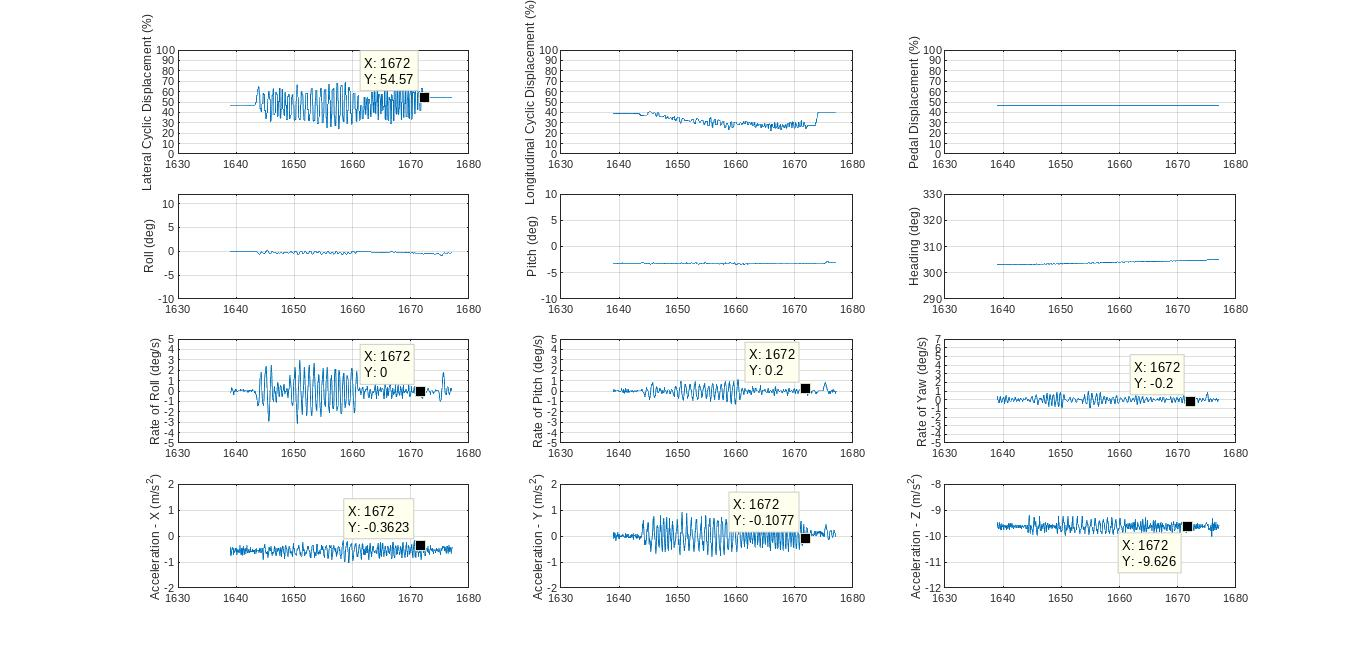
\includegraphics[width=1\linewidth]{gambar/Max_dr.jpg}
	\caption{Grafik data pengukuran waktu peluruhan amplitudo pada variasi FLLA kondisi-3 yang berakhir pada detik ke-1672.}
	\label{fig:FLLA-3}
\end{figure}

Sebagai salah satu bagian dari pengujian, akan diberikan perhitungan untuk variasi FLLA pada kondisi 3, dimana pada kondisi dan variasi tersebut memiliki waktu peluruhan yang paling lama. Grafik pada kondisi dan variasi yang dimaksud dapat dilihat pada gambar \ref{fig:FLLA-3}.
 
Grafik pada gambar \ref{fig:FLLA-3} merupakan grafik yang telah dipotong sesuai dengan interval \textit{input} yang diberikan. \textit{Input lateral} yang diberikan berakhir pada detik ke-1672, akan tetapi helikopter masih memberikan respon getaran. Walau demikian, respon getaran yang diberikan memiliki bentuk yang tidak dapat diidentifikasi, sehingga untuk dapat menghitung nilai \textit{logarithmic decrement} diperlukan pendekatan secara detail terhadap nilai puncak dan lembah dari grafik yang dimiliki oleh respon helikopter.

\subsection{Hasil pengukuran getaran pada Akselerometer}

Data hasil pengukuran pada akseleromter akan dibandingkan dengan acuan dari MIL-STD-810H-Method-514.8 (vibrasi). Dari grafik gambar \ref{fig:MIL_STD} yang berupa tabel didapatkan batas siklus osilasi helikopter Maka didapatkan grafik batas siklus osilasi pada gambar \ref{fig:batas_siklus}.

\begin{figure}[H]
	\centering
	\fbox{\includegraphics[width=0.8\linewidth]{/run/media/hadi/Abdul_Hadi/HADI_2.0/THOLABUL_ILMI/KP_TA/TA/Progres/Oscillation_cycle_limit.jpg}}
	\caption{Grafik batas siklus osilasi dari acuan MIL-STD-810H-Method-514.8 (vibrasi).}
	\label{fig:batas_siklus}
\end{figure}

Grafik pada gambar \ref{fig:batas_siklus} didapatkan dengan menghitung sumber frekuensi dari rotor helikopter. Informasi dari PTDI memberikan nilai kecepatan maksimum dan minimum dari rotor berturut-turut adalah sebesar $365 rpm$ dan $355 rpm$, sehingga didapatkan frekuensi ($f_1$) nya adalah dimulai dari $5.92 Hz$ (minimum) hingga $6.08 Hz$ (maksimum). Perhitungan nilai $f_2$, $f_3$, dan $f_4$ dapat dilihat pada tabel \ref{tb:batas_siklus}. Nilai peak pada tabel tersebut dihitung menggunakan formulasi yang terletak pada kolom "\textbf{PEAK ACCELERATION ($A_x$) at $f_x$ (GRAVITY UNITS (g))}".

Berikut ini merupakan data hasil akselerometer berdasarkan variasi dan kondisi yang telah diberikan pada tabel \ref{tb:variasi_input} dan tabel \ref{tb:variasilanding}.

\begin{figure}[H]
	\centering
	\fbox{\includegraphics[width=0.8\linewidth]{/run/media/hadi/Abdul_Hadi/HADI_2.0/THOLABUL_ILMI/KP_TA/TA/Progres/Helicopter_response_image/Config_11/5_Config_11_FLLO.jpg}}
	\caption{Hasil pengukuran respon frekuensi kondisi-11 pada variasi FLLO.}
	\label{fig:11_FLLO}
\end{figure}

Grafik pada gambar \ref{fig:11_FLLO} merupakan grafik dengan nilai respon terbesar dibandingkan respon-respon dari kondisi dan variasi yang telah dilakukan, yaitu dengan amplitudo sebesar 0.143 g-peak pada frekuensi 23.74$Hz$. 

\begin{table}[]
	\caption{Tabel perhitungan batas siklus osilasi.}
	\label{tb:batas_siklus}
	\centering
	\begin{tabular}{|ccc|cc|}
		\hline
		\multicolumn{3}{|c|}{Frekuensi (Hz)}                                                       & \multicolumn{2}{c|}{Peak (g)}             \\ \hline
		\multicolumn{1}{|c|}{$f_1$ lower} & \multicolumn{1}{c|}{5.92}  & \multirow{2}{*}{$1p$}       & \multicolumn{1}{c|}{$A_1$ lower} & 0.1464 \\ \cline{1-2} \cline{4-5} 
		\multicolumn{1}{|c|}{$f_1$ upper} & \multicolumn{1}{c|}{6.08}  &                           & \multicolumn{1}{c|}{$A_1$ upper} & 0.1515 \\ \hline
		\multicolumn{1}{|c|}{$f_2$ lower} & \multicolumn{1}{c|}{23.68} & \multirow{2}{*}{$1p*n$}   & \multicolumn{1}{c|}{$A_2$ lower} & 2.368  \\ \cline{1-2} \cline{4-5} 
		\multicolumn{1}{|c|}{$f_2$ upper} & \multicolumn{1}{c|}{24.32} &                           & \multicolumn{1}{c|}{$A_2$ upper} & 2.432  \\ \hline
		\multicolumn{1}{|c|}{$f_3$ lower} & \multicolumn{1}{c|}{47.36} & \multirow{2}{*}{$1p*n*2$} & \multicolumn{1}{c|}{$A_3$ lower} & 1.764 \\ \cline{1-2} \cline{4-5} 
		\multicolumn{1}{|c|}{$f_3$ upper} & \multicolumn{1}{c|}{48.64} &                           & \multicolumn{1}{c|}{$A_3$ upper} & 1.636  \\ \hline
		\multicolumn{1}{|c|}{$f_4$ lower} & \multicolumn{1}{c|}{71.04} & \multirow{2}{*}{$1p*n*3$} & \multicolumn{1}{c|}{$A_4$ lower} & 1.5    \\ \cline{1-2} \cline{4-5} 
		\multicolumn{1}{|c|}{$f_4$ upper} & \multicolumn{1}{c|}{72.96} &                           & \multicolumn{1}{c|}{$A_4$ upper} & 1.5    \\ \hline
	\end{tabular}
\end{table}

\subsection{Hasil Perhitungan}

Berdasarkan matriks yang telah didapatkan pada persamaan \ref{eq:linearisasi} kemudian disubtitusi pada persamaan \ref{eq:EOM} dan diubah menjadi bentuk \textit{state-space} pada persamaan \ref{eq:state-space_simplified}.

\begin{equation}
	\mathbf{A}=\begin{bmatrix}
	\mathbf{0}& \mathbf{I}\\
	\mathbf{-M}^{-1}\mathbf{K}& \mathbf{-M}^{-1}(\mathbf{C}+\mathbf{G})
	\end{bmatrix}
\end{equation}

Dikarenakan informasi material helikopter belum diketahui, maka dilakukan pendekatan untuk nilai propertis persamaan diatas, dimana untuk masing-masing propertis adalah sebagai berikut:

\begin{table}[H]
	\centering
	\caption{Pendekatan nilai propertis helikopter.}
	\label{tb:propertis}
	\begin{tabular}{|c|c|c|}
		\hline
		Variabel     & Nilai  	& Besaran \\ \hline
		$L$          & 5.97  	& $m$     \\ \hline
		$k_y$        & 44.100  	& $N/m$   \\ \hline
		$m_y$        & 4.500   	& kg      \\ \hline
		$c_y$        & 441    	& $Ns/m$  \\ \hline
		$m_{\delta}$ & 100.5  	& kg      \\ \hline
		$k_{\delta}$ & 89.028  	& $N/m$   \\ \hline
		$c_{\delta}$ & 106.92 	& $Ns/m$  \\ \hline
	\end{tabular}
\end{table}

Nilai eigen dapat diperhitungkan dari matriks $\mathbf{A}$. Dari hasil tersebut, didapatkan 6 solusi nilai eigen saat kondisi natural, yaitu saat $\tilde{S}_c = \tilde{S}_d = 0$ (tidak saling berhubungan / \textit{uncoupled}). Sehingga dari kondisi tersebut didapatkan grafik bagian imajiner terhadap kecepatan rotor $\Omega$ dan didapatkan pula bagian rill terhadap kecepatan rotor $\Omega$.

\begin{figure}[H]
	\centering
	\fbox{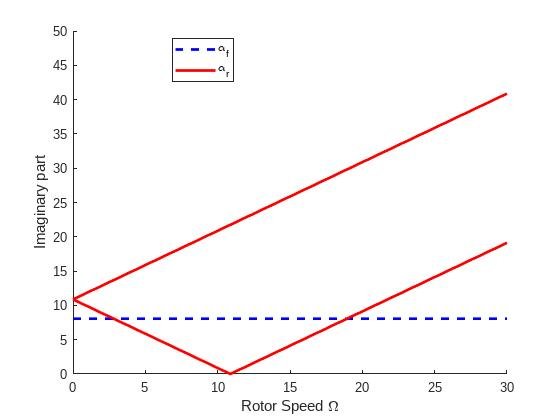
\includegraphics[width=0.8\linewidth]{gambar/Imag(uncoupled).jpg}}
	\caption{Plot grafik imajiner terhadap kecepatan rotor $\Omega$ pada kondisi \textit{uncoupled}.}
	\label{fig:imag(uncoupled)}
\end{figure}

\begin{figure}[H]
	\centering
	\fbox{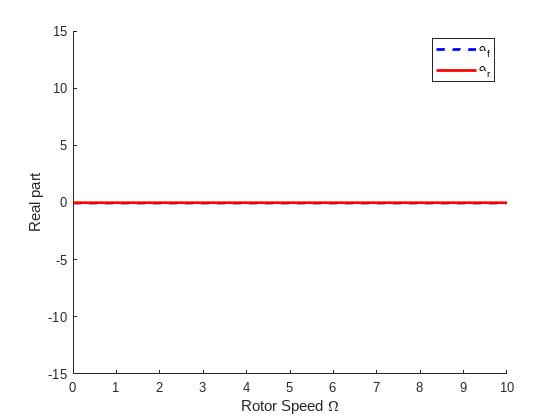
\includegraphics[width=0.8\linewidth]{gambar/Real(uncoupled).jpg}}
	\caption{Plot grafik real terhadap kecepatan rotor $\Omega$ pada kondisi \textit{uncoupled}.}
	\label{fig:real(uncoupled)}
\end{figure}

Kemudian, berikut ini adalah grafik plot untuk bagian imajiner dan riil saat sistem \textit{coupled}.

\begin{figure}[H]
	\centering
	\fbox{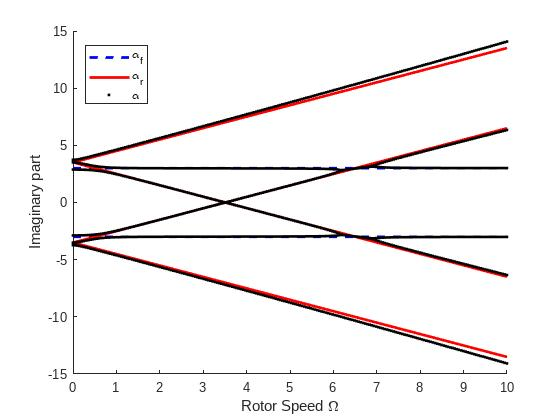
\includegraphics[width=0.8\linewidth]{gambar/Imag(coupled).jpg}}
	\caption{Plot grafik imajiner terhadap kecepatan rotor $\Omega$ pada kondisi \textit{coupled}.}
	\label{fig:imag(coupled)}
\end{figure}

\begin{figure}[H]
	\centering
	\fbox{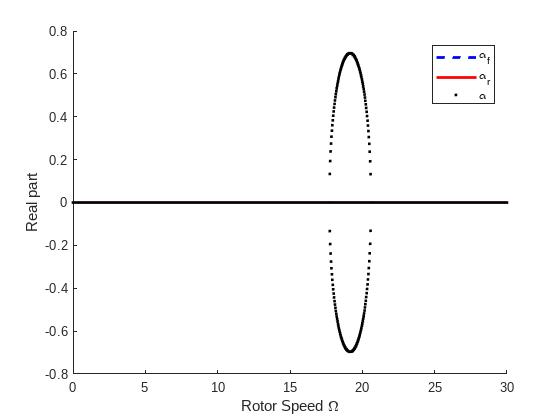
\includegraphics[width=0.8\linewidth]{gambar/Real(coupled).jpg}}
	\caption{Plot grafik real terhadap kecepatan rotor $\Omega$ pada kondisi \textit{coupled}.}
	\label{fig:real(coupled)}
\end{figure}

$\alpha_f$ merupakan nilai eigen dari \textit{fuselage} (berwarna biru dengan garis putus-putus) dan $\alpha_r$ merupakan nilai eigen dari rotor helikopter (berwarna merah). Sedangkan $\alpha$ merupakan nilai eigen dari sistem \textit{coupled}.

\section{Pembahasan}
\label{sec:pembahasan}
